\documentclass[]{report}


\usepackage{blindtext}
\usepackage{titlepic}
\usepackage{titlesec}
\usepackage{graphicx}
\usepackage{float}
\usepackage{titlesec}
\usepackage{listings}
\usepackage[%  
colorlinks=true,
pdfborder={0 0 0},
linkcolor=red
]{hyperref}

\makeatletter
\renewcommand{\@makechapterhead}[1]{%
	\vspace*{50 pt}%
	{\setlength{\parindent}{0pt} \raggedright \normalfont
		\bfseries\Huge
		
		#1\par\nobreak\vspace{40 pt}}}
\makeatother

% Title Page
\title{COSC 3P98 Assignment 3}
\author{Brett Terpstra - 6920201 - bt19ex@brocku.ca}
\titlepic{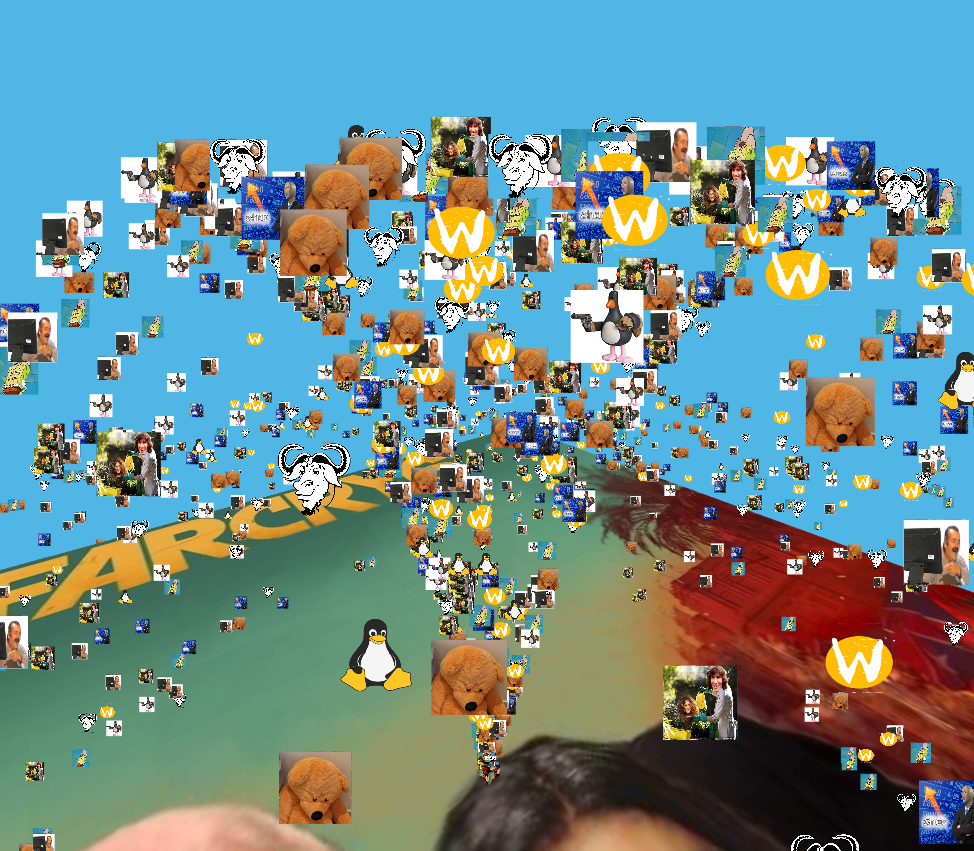
\includegraphics[width=\textwidth]{screenshot001.png}}
\renewcommand*\contentsname{Table Of Contents}



\begin{document}
\maketitle

\begin{abstract}
Particle systems are the cornerstone of all modern game engines as they allow effects such as smoke which are otherwise impossible with static meshes. Ergo a good particle system should be flexible while maintaining stable performance. This document serves as an informal report on the design and implementaion of two particle systems; a basic but flexible engine and a high performance extendable "modern" GPU powered particle system.
\end{abstract}

\tableofcontents

\chapter{Introduction}
\section{Description}
Over the course of working on this assignment I began to wonder how far I could push my hardware and \autoref{chap:hp} "Performance Mode" will go furher into this. As for the main assignment requirements, they are met simply by running the CMake project. On my hardware the simple particle fountain can reach 30k particles and features sorted transparency.
\subsection{Extra Features}
\begin{itemize}
	\item Ordered Alpha Blending
	\item "Spray" Mode (12)
	\item Textured Particles/Plane/Cube (16)
	\item Particles with Different Textures (18)
	\item Extra Feature - "Performance Mode" (23)
\end{itemize}
\subsection{Missing Features}
Random spin mode was left out intentionally for two reasons. One, I specifically designed the particle strucutre to fit in 32 bytes, half the width of a cache line. Two, the potential marks was not worth disturbing the particle data structure and further altering the particle system. There is likely little benefit to ensuring the particles fit nicely inside a cache line as most of the CPU time is spent on OpenGL API calls. See \autoref{chap:hp} "Performance Mode" for more information.
\section{Building}
As of writing this report, I have yet to build and test on Windows. The Visual Studio project will build without issues, however, since this assignment was primarily designed and tested on Debain 12 "Bookworm" (Linux 6.1.0-6-amd64) using AMD/Intel hardware (Mesa 22.3.6), I reccomend using CMake. 
\subsection{Caveats}
The assignment makes use of a non-standard OpenGL extention during texture loading. "GL\_TEXTURE\_MAX\_ANISOTROPY\_EXT" should work on all modern Intel/AMD/Nvidia hardware, if it doesn't work on your hardware consider removing the line from texture.h and high\_perf.cpp
\subsection{Build Commands}
\begin{figure}[H]
	\centering
	\begin{lstlisting}
	mkdir build && cd build
	cmake -DCMAKE_BUILD_TYPE=Release ../
	make -j 16
	./assign3
	\end{lstlisting}
	\caption{Linux build commands.}
\end{figure}
\section{Usage}
Keybindings and usage instructions are printed at program startup.

\chapter{Performance Mode}\label{chap:hp}
\subsection{Design}
The high performance mode is the result of a weekend hack-a-ton where I wanted to see how easy it would be to implement a million particle+ renderer. The rendering engine itself can handle around 20 million particles at about 60fps (\autoref{fig:screenshot002}).

\begin{figure}[H]
	\centerline{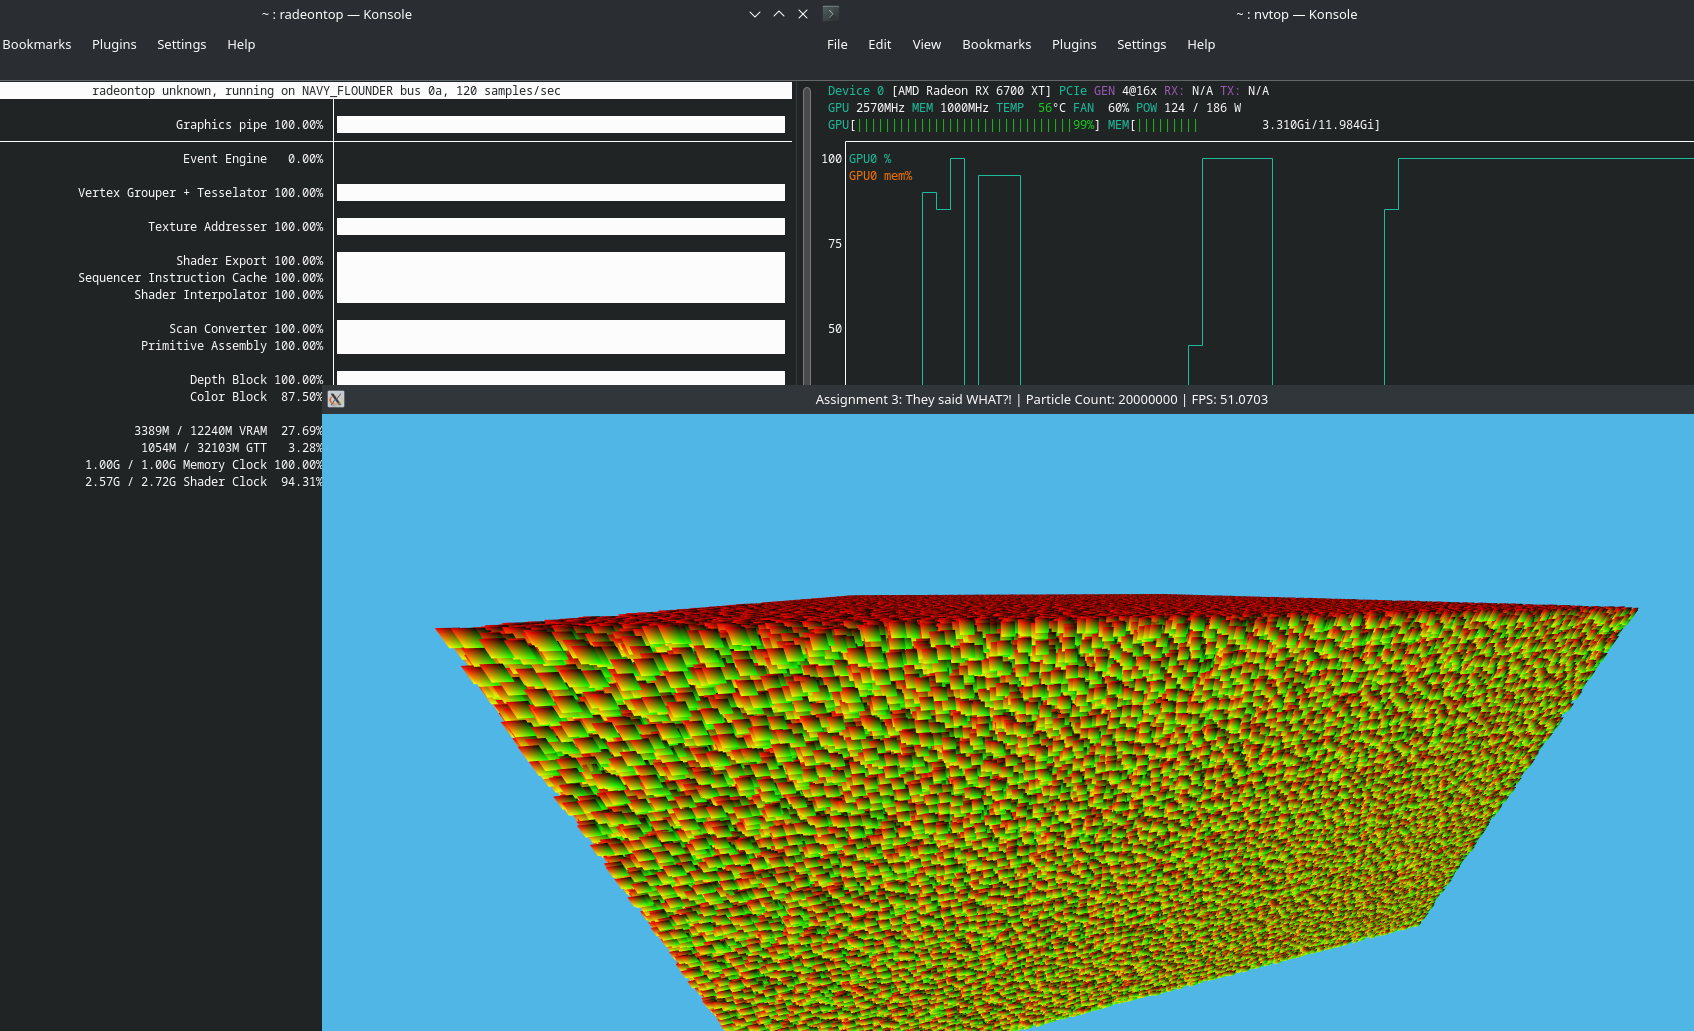
\includegraphics[width=1.5\linewidth]{screenshot002}}
	\caption[]{20 million particles distributed in a 50x25x50 cube with load monitors}
	\label{fig:screenshot002}
\end{figure}


\end{document}          
